%TODOS FOR THIS LAB
%
%1.  This is too long.  Have them do Prims or Kruskalls, but not both
%2.  Compare their implemented solution to NetworkX
%3.  More examples of the different kinds of graphs mentioned in the introduction, or otherwise don't mention them at all.


\lab{Algorithm}{Kruskal's and Prim's Algorithm}{Kruskal's and Prim's Algorithm}
\label{Ch:Kruskal}

\objective{Find a minimum spanning tree for a connected weighted graph using Kruskal's Algorithm and Prim's Algorithm.}

\section*{Weighted Graphs and Spanning trees}

Remember that a graph is composed of two sets, a set of nodes and a set of edges that connect these nodes. 

\begin{figure}[H]
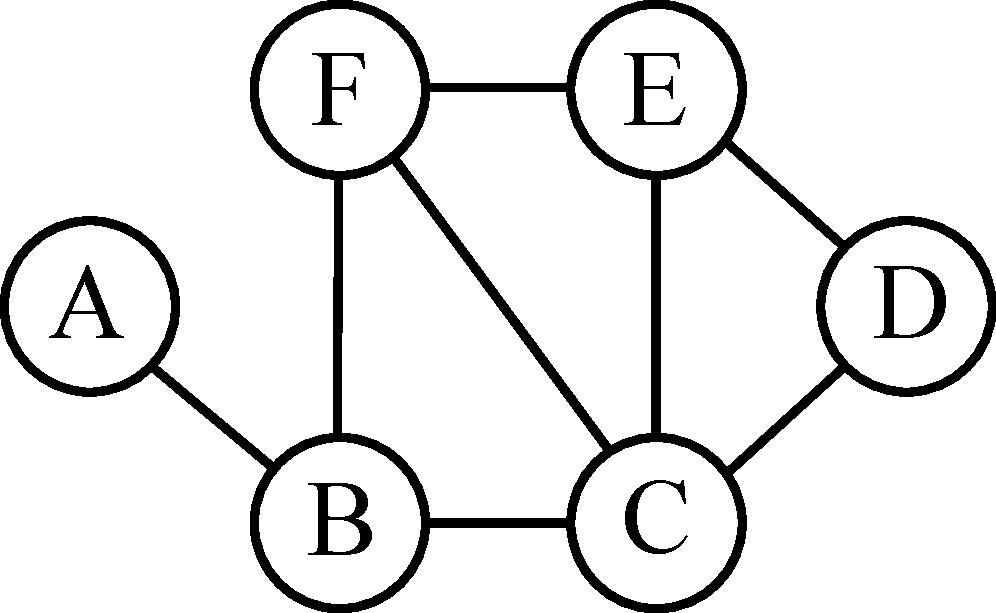
\includegraphics[width = .4\textwidth]{graph1.pdf}
\caption{An example of a graph}
\label{mst:graph1}
\end{figure}

A graph is directed if connections are uni-directional, and undirected if they are bi-directional.
Figure \ref{mst:graph1} shows an undirected graph.
%A weighted graph is a graph where each edge has a value associated with it.
%Usually these values represent some sort of cost or distance.
A connected graph is a graph where there is a path, or a set of edges, that connect every two nodes together.
We can write a matrix that describes this type of graph.
We let each row of our matrix represent a starting point and each column represent a destination.
If an edge from one node to another exists, we put the weight of the edge.
If there is no edge, we put a 0.
For the above graph we generate the following matrix:

\[
A = \begin{pmatrix}
0 & 1 & 0 & 0 & 0 & 0\\
1 & 0 & 1 & 0 & 0 & 1\\
0 & 1 & 0 & 1 & 1 & 1\\
0 & 0 & 1 & 0 & 1 & 0\\
0 & 0 & 1 & 1 & 0 & 1\\
0 & 1 & 1 & 0 & 1 & 0\\
\end{pmatrix}
\]

This matrix is called an adjacency matrix.
Note that this matrix is symmetric, since the graph is undirected. 

Now consider the graph in Figure \ref{mst:graph4}.  This graph is the same as the graph in Figure \ref{mst:graph1}, except now there is a weight attached to each edge.  The matrix for this graph is
\[
A = \begin{pmatrix}
0 & 3 & 0 & 0 & 0 & 6\\
3 & 0 & 5 & 0 & 0 & 4\\
0 & 5 & 0 & 1 & 1 & 5\\
0 & 0 & 1 & 0 & 2 & 0\\
0 & 0 & 1 & 2 & 0 & 4\\
6 & 4 & 5 & 0 & 4 & 0\\
\end{pmatrix}
\]

Another way to store the information from a graph is to make a list of the edges with their corresponding weights.
For an unweighted undirected graph, this would just mean making a list of the pairs of nodes that correspond to each edge.
For a weighted undirected graph a third value could be added to the end of each edge representing the corresponding weight of that edge.
A list like this for the graph in Figure \ref{mst:graph1} would look like this:

\begin{align*}
[('A', 'B'),
 ('B', 'C'),
 ('B', 'E'),
 ('B', 'F'),
 ('C', 'D'),\\
 ('C', 'E'),
 ('C', 'F'),
 ('D', 'E'),
 ('E', 'F')]
\end{align*}

For this lab, we will be focusing on undirected weighted graphs.

A spanning tree of a connected undirected graph $G$ is an undirected graph that contains all the nodes of $G$, a subset of the edges, and no cycles.
A cycle, for undirected graphs, is a path where you start and end on the same node without crossing any edge more than once.
Figure \ref{mst:graph3} shows a cycle in an undirected graph.

\begin{figure}[H]
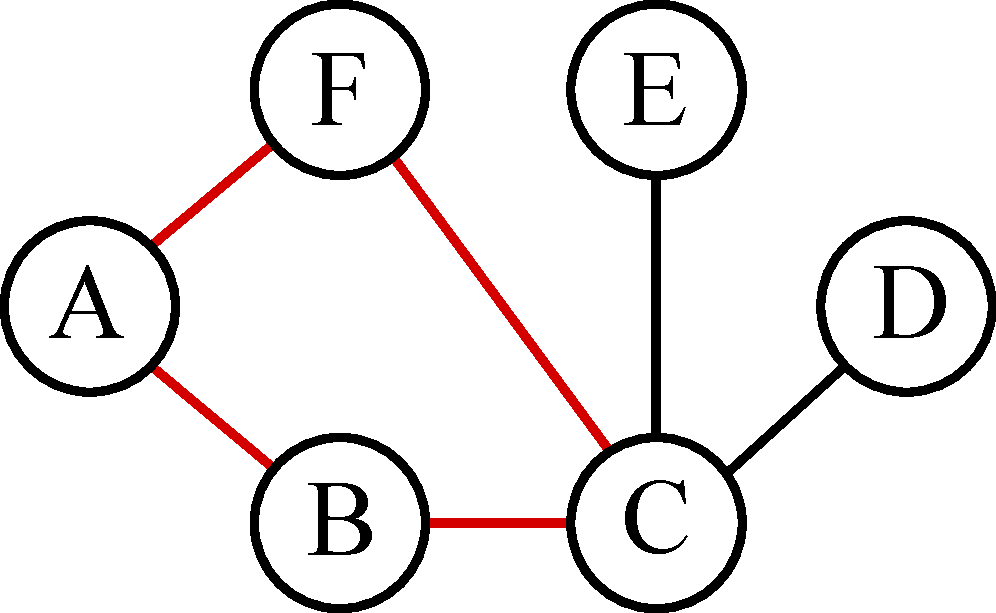
\includegraphics[width = .4\textwidth]{graph3.pdf}
\caption{A cycle in an undirected graph}
\label{mst:graph3}
\end{figure}

The minimum spanning tree (MST) of a weighted undirected graph is a spanning tree where the sum of the weights of the subset of edges is less than or equal to the sum of the weights of every other spanning tree.
Both Kruskal's and Prim's Algorithms are methods that find the minimum spanning tree of a weighted directed graph.
Figure \ref{mst:graph2} shows a minimum spanning tree of the graph shown in \ref{mst:graph1}.

\begin{figure}[H]
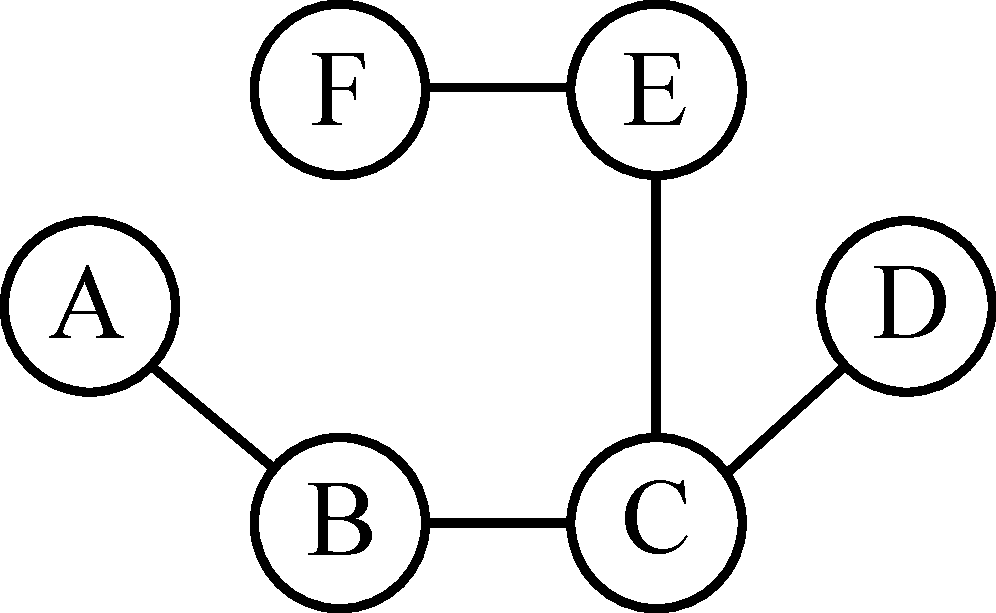
\includegraphics[width = .4\textwidth]{graph2.pdf}
\caption{A minimum spanning tree for the graph in Figure \ref{mst:graph1}.}
\label{mst:graph2}
\end{figure}

\begin{figure}[H]
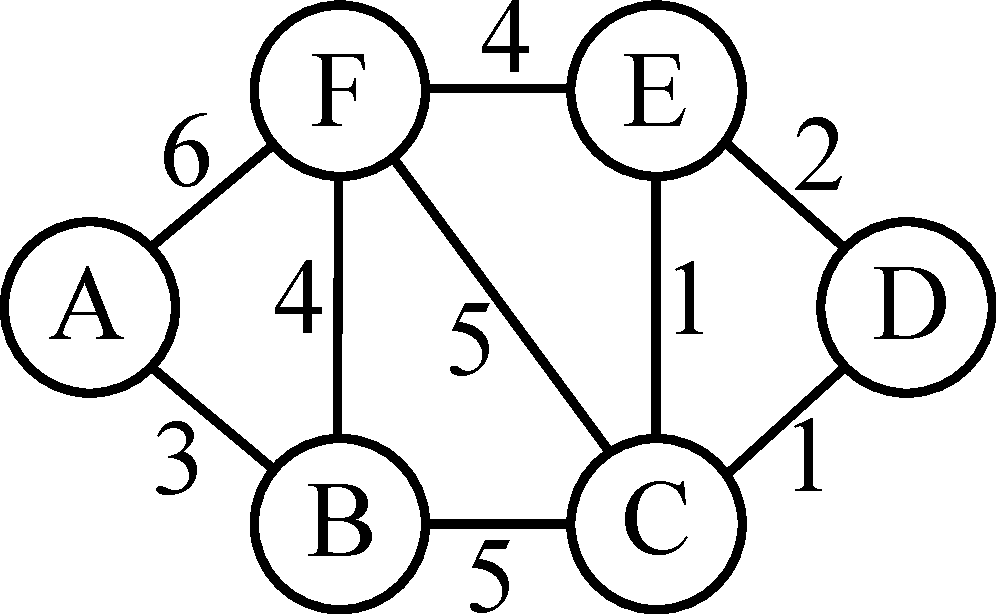
\includegraphics[width = .4\textwidth]{graph4.pdf}
\caption{A weighted undirected graph}
\label{mst:graph4}
\end{figure}

\begin{figure}[H]
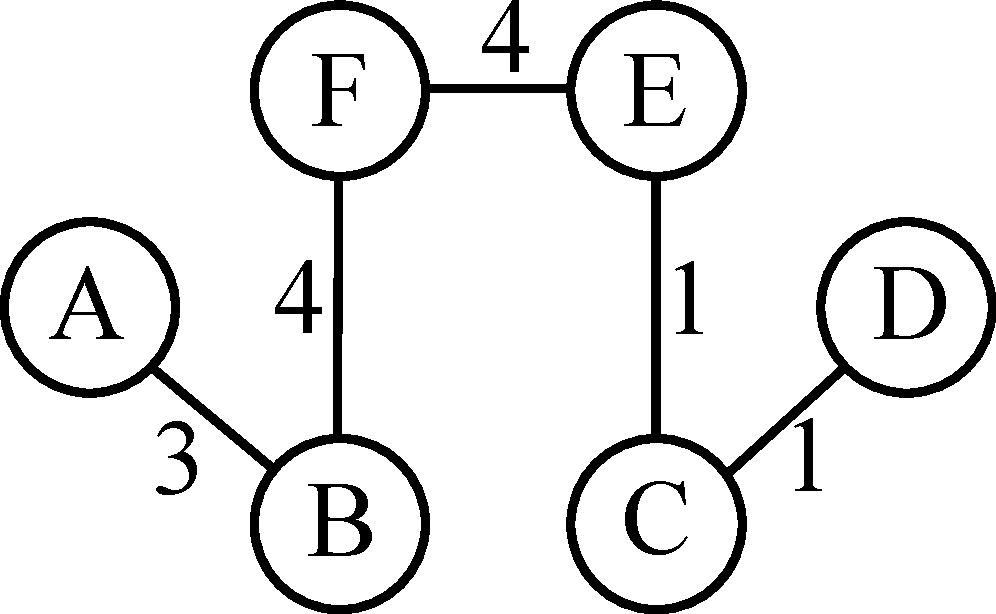
\includegraphics[width = .4\textwidth]{graph5.pdf}
\caption{The MST of the graph in Figure \ref{mst:graph4}.}
\end{figure}

\section*{Kruskal's algorithm}

Given a weighted directed graph G with $n$ nodes, Kruskal's algorithm finds a minimum spanning tree by sorting the edges from smallest to largest then, starting from the smallest, the algorithm adds edges to the tree as long as the addition of each new edge does not create a cycle.
When $n-1$ edges have been added, the algorithm stops.

In order to avoid creating cycles while building the tree, it is necessary to keep track of which portions of the tree currently lie in connected groups.
This can be done by creating a dictionary where, when the algorithm starts, each node points to itself as the "root" of its own tree.
As you add edges to the tree you will change which nodes are the "root" nodes to track which nodes are currently connected.
Doing it in this way lets you run the algorithm by iterating over the edges by weight in ascending order, adding them to the tree if they connect nodes that are not already connected by the current tree.

Consider the graph in Figure \ref{mst:graph4}.
Applying Kruskal's algorithm, the first step to finding a minimum spanning tree is to sort the edges by weight.
The result is something like the list \li{[(C, D, 1), (C, E, 1), (D, E, 2), (A, B, 3), (B, F, 4), (E, F, 4), (B, C, 5), (C, F, 5), (A, F, 6)]}.
We initialize our tree to be an empty list \li{[]}.
To track the root nodes of each tree, we will also initialize a dictionary where each node points to itself.
It will look like this: \li{\{A:A, B:B, C:C, D:D, E:E, F:F\}}.
Since there are 6 nodes in the graph, we will continue until we have 5 edges in the tree.

Now we begin iterating through the edges to build the tree.
The first edge in the list is \li{(C,D,1)}.
The root for \li{C} is \li{C} and the root for \li{D} is \li{D}, so we add this edge to the tree.
The tree becomes \li{[(C, D, 1)]}.
We then change the root node of \li{D} to be \li{C}.
The dictionary of root nodes now looks like \li{\{A:A, B:B, C:C, D:C, E:E, F:F\}}.

Now we process the next edge, \li{(C, E, 1)}.
The root node of \li{C} is \li{C}, and the root node of \li{E} is \li{E}, so adding this edge does not create a cycle.
We add this edge into the tree, so the tree is now \li{[(C, D, 1), (C, E, 1)]}.
Then we change the root of \li{E} so that it is \li{C}, so the dictionary is \li{\{A:A, B:B, C:C, D:C, E:C, F:F\}}.

The next edge is \li{(D, E, 2)}.
The root node of the tree containing \li{D} is \li{C} and the root node of the tree containing \li{E} is \li{C}, so these nodes are already connected, so we do not add this edge to the tree.

The next ege is \li{(A, B, 3)}.
The root node for \li{A} is A, and the root node for \li{B} is \li{B}, so we add the edge to the tree and update the dictionary.
The dictionary becomes \li{\{A:A, B:A, C:C, D:C, E:C, F:F\}}

The next edge is \li{(B, F, 4)}.
The root node for \li{B} is \li{A} and the root node for \li{F} is \li{F}, so we add the edge to the tree and change the root node of \li{F} to be \li{A}.
The dictionary becomes \li{\{A:A, B:A, C:C, D:C, E:C, F:A\}}

The next edge is \li{(E, F, 4)}.
The root node for \li{E} is \li{C} and the root node for \li{F} is \li{A}.
We add the edge to the tree and end the algorithm since there are now 5 edges in the tree.
If we were to continue the algorithm, we would update the root node of \li{A} to be \li{C}.

Notice how we just updated the root of the root node for one of the nodes in the edge we just added.
Managing the root nodes in this way makes it so that, in order to find the root node of \li{F}, we must trace back through the dictionary until we find a node that points to itself.
For example, the way we would now find the root node of \li{F} is to get the value for \li{F} from the dictionary, which is \li{A}, then get the value for \li{A} from the dictionary, which is \li{C}.
The value of \li{C} in the dictionary is itself, so it is the root node of the graph containing \li{F}.
It is necessary to trace through the dictionary in this manner each time to find the root nodes we need at each iteration because it lets us avoid iterating over all of the nodes and updating their root values each time.

Here is the pseudocode for the algorithm as we have described it above:

\begin{itemize}

% Note: The comments in the solutions match the pseudocode.
% When making changes, pleas keep that in mind.

\item Initialize an empty list of edges for the minimum spanning tree.

\item Make a dictionary that points each node toward its root (not always directly to it).
Start with each node pointing to itself.

\item Initialize the number of nodes that still need to be processed to the number of nodes minus 1.

\item Define a helper function that, given a node, traces through the dictionary to find the root of its tree.
This can be done like this:

	\begin{itemize}

	\item Initialize a temporary variable to be the node for which we are finding the root.

	\item While the temporary node does not point to itself in the dictionary:

		\begin{itemize}

		\item Update the temporary node to be the node it currently points to in the dictionary.

		\end{itemize}

	\item Return the temporary node.

	\end{itemize}

\item Iterate over the edges by ascending weight.
Use a \li{for} loop for this and return the tree when it is big enough.
That will break the loop for you.

	\begin{itemize}

	\item Trace through the dictionary to find the root node of each of the nodes in the edge you are processing.

	\item If the roots are not the same (i.e. if adding the edge doesn't form a cycle):

		\begin{itemize}

		\item Add the edge to the tree.

		\item Lower the number of edges remaining by one.

		\item If the number of edges remaining is 0, return the tree (which also breaks the loop).

		\item Update the root of the root of the second node in the edge to be the root of the first node in the edge.
			This lets us record that the two subtrees are now connected.

		\end{itemize}

	\end{itemize}

\end{itemize}
Note on implementation: You can iterate over a sorted copy of a list using the built in \li{sorted} function.
You can sort by the third value in each tuple using the \li{itemgetter} function that is part of the \li{operator} library included with Python.
For example:
\begin{lstlisting}
from operator import itemgetter
...
for n1, n2, weight in sorted(edges, key=itemgetter(2)):
    ...
\end{lstlisting}

\begin{problem}
Implement Kruskal's algorithm.
Test your algorithm on random symmetric arrays.
You can generate a random symmetric array by multiplying a random array by its transpose.
Use the data from MSTdata.npy to test your tree.
Use np.load("MSTdata.npy") to get it.
Use the \li{formChanger} function below to put it in the right form.
\begin{lstlisting}
\end{lstlisting}
def formChanger(oldData):
    newData=[] for i in oldData: newData.append((i[0],i[1],int(i[2])))
    return newData
\end{problem}
\section*{Prim's algorithm}

Prim's is a similar algorithm for finding minimum spanning trees.
It  is much slower than Kruskal's algorithm for sparse graphs, but is much faster for dense graphs.
The order of complexity of Kruskal's algorithm is $\mathcal{O}\left( m \log{n} \right)$ where $m$ is the number of edges and $n$ is the number of nodes.
If the graph is completely dense, then $m=n^2$ and this order becomes $\mathcal{O}\left( n^2 \log{n}\right)$.
The best sorting algorithms are $\mathcal{O}\left( m \log{m}\right)$ for $m$ items, so the best we can do while still sorting the edges is $\mathcal{O}\left( n^2 \log{n^2}\right) = 2 \mathcal{O}\left( n^2 \log{n}\right) = \mathcal{O}\left( n^2 \log{n} \right)$.
Prim's algorithm avoids sorting the edges and has complexity $\mathcal{O} \left( n^2 \right)$.

The way Prim's algorithm works is that it starts with one node and, node by node, builds a tree containing all the nodes in the graph.
At each iteration it adds to the tree the shortest edge that runs from a processed node to an unprocessed node.
Since the algorithm needs to quickly find the nodes that share an edge with each node, it will be good to make a dictionary that maps each node to a list of all the edges that contain it.
The smallest edge in the graph can be a good place to start the algorithm.
While we construct the dictionary we need, we can also find the smallest edge.

Again, consider the example shown in Figure \ref{mst:graph4}.
We first initialize a dictionary with all the nodes as keys to track which of all the nodes have not been processed.
At the beginning it will be \li{\{A:False, B:False, C:False, D:False, E:False, F:False\}}.
We then form the dictionary that maps each node to the edges that contain it.
Since we will already know one node of each edge while we use the dictionary, we only need to store the node that is not being looked up.
It will be \li{\{A:[(B, 3), (F, 6)], B:[(A, 3), (C, 5), (F, 4)], C:[(B, 5), (D, 1), (E, 1), (F, 5)], D:[(C, 1), (E, 1)], E:[(C, 1), (D, 2), (F, 4)], F:[(A, 6), (B, 4), (C, 5), (E, 4)]\}}.
We will also initialize an empty dictionary to track the shortest edges that run between nodes we have processed and nodes that we haven't.
As we iterated over the the edges in our initialization step we were also able to find the shortest edge.
In this case, it is either \li{(D, C, 1)} or \li{(D, E, 1)}.
Say we are starting with \li{(D, C, 1)}.
We now initialize our tree as the list \li{[(D, C, 1)]}.
Once that is done, we mark \li{D} and \li{C} as processed in the dictionary that tracks which nodes have been processed.
Now we start to build our dictionary of nodes that are one edge away from the nodes we have already processed.
In this case, after adding the shortest edges between processed and unprocessed nodes to the dictionary, the dictionary becomes \li{\{B:(C, B, 5), E:(C, E, 1), F:(C, F, 5)\}}.
Notice how we did not include \li{E:(D, E, 2)} since there is a shorter edge to \li{E} from \li{C}.

Of the edges in the dictionary of edges that can be processed next, the shortest is \li{(C, E, 1)}, so we add that edge to the tree and mark \li{E} as processed.
With \li{E} being processed, we can now reach \li{F} at a cost of 4.
After making this change, the dictionary of edges to process becomes \li{\{B:(C, B, 5), E:(C, E, 1), F:(E, F, 4)\}}.
Since \li{E} no longer needs to be processed, we can remove it from consideration, so we modify this dictionary again so it becomes \li{\{B:(C, B, 5), F:(E, F, 4)\}}.

Of the edges to be processed next, \li{(E, F, 4)} is the shortest, so we add it to the tree and mark \li{F} as processed.
After performing the appropriate modifications to the dictionary of edges to be processed next, it becomes \li{\{B:(F, B, 4), A:(F, A, 6)\}}.

Of the edges to be processed next, \li{(F, B, 4)} is the shortest, so we add it to the tree and mark \li{B} as processed.
After performing the appropriate modifications to the dictionary of edges to be processed next, it becomes \li{\{A:(B, A, 3)\}}.

The only edge to be considered is \li{(B, A, 3)}, so we add that to the tree.
The tree is long enough that it it spans the nodes, so the algorithm is finished.

Here's pseudocode for a version of Prim's algorithm.
It isn't a perfectly optimized version, but it is pretty good.

\begin{itemize}

% Note: The comments in the solutions match the pseudocode.
% When making changes, pleas keep that in mind.

\item Initialize a dictionary to track which nodes have been processed.

\item Initialize an empty dictionary of lists to track the edges containing each node.

\item Fill the edge list.
	Be sure to add each edge to the list corresponding to both of its nodes.

\item Get the first edge to add (It can be the shortest edge from any given node, the shortest edge is a good pick).

\item Mark the nodes in the first edge as processed.

\item Initialize the tree to be the list containing the first edge.

\item Initialize an empty dictionary that will be used to contain the edges that can be processed next.

\item Define a helper function to insert an edge into the dictionary  if that insertion is needed.
	That can be done like this:

	\begin{itemize}

	\item Get the value of the node that is reached by the edge.

	\item If that node isn't in the dictionary, set its value to be the edge passed to the functions.

	\item If it is in the dictionary already, set its value to be the shorter of the edge being processed and the edge already in the dictionary.

	\end{itemize}

\item Use the helper function to insert the edges reached by the first two processed nodes into the dictionary of edges to be processed.

\item Until the tree contains enough edges to span all the nodes:

	\begin{itemize}

	\item Find the shortest edge in the dictionary of edges to be processed.

	\item Remove the shortest edge from the dictionary.

	\item Add it to the tree.

	\item Mark the node reached by the new edge as processed.

	\item Use the helper function to insert the edges reached by the newly processed node into the dictionary of edges to be processed.

	\end{itemize}

\item Return the completed tree.

\end{itemize}

\begin{problem}
Write a Python function that uses Prim's algorithm to find the minimum spanning tree of a graph.
Test your implementation with the same data as the previous problem.
Compare the speed of Prim's algorithm with the speed of Kruskal's algorithm.
\end{problem}

Many graph packages have functions for finding the minimal spanning tree. One of these is NetworkX. You begin as follows
\begin{lstlisting}
import networkx as nx
G=nx.Graph()
\end{lstlisting}
You can add a node $x$ with \li{G.add_node(x)} and add a edge from $x$ to $y$ with weight n with \li{G.add_edge(x,y,weight=n)}. Then \li{nx.minimum_spanning_tree(G)} returns the minimal spanning tree using Kruskals algorithm.

\begin{problem}
Use NetworkX to find the minimal spanning tree of the data in MSTdata.npy. Compare the output with that of your algorithm.
\end{problem}
